\documentclass[12pt, letterpaper]{article}
\usepackage{amsmath}
\usepackage{amssymb}
\usepackage[finnish,english]{babel}
%\usepackage{biblatex}
\usepackage{braket}
\usepackage{fancyhdr}
\usepackage{geometry}
\usepackage{graphicx}
\usepackage{listings}
\usepackage{mathtools}
\usepackage{paracol}
\usepackage{physics}
\usepackage{titlesec}
\usepackage{tikz-feynman}
\usepackage{import}
\usepackage{xifthen}
\usepackage{pdfpages}
\usepackage{transparent}
\usepackage[many]{tcolorbox}
\usepackage{clara}
%\usepackage[T1]{fontenc}

%\addbibresource{sources.bib}

\newcommand{\N}{\mathbb{N}}
\newcommand{\Z}{\mathbb{Z}}
\newcommand{\Q}{\mathbb{Q}}
\newcommand{\R}{\mathbb{R}}
\newcommand{\C}{\mathbb{C}}

\newcommand{\incfig}[2][1]{%
  \def\svgwidth{#1\columnwidth}
  \import{./figures/}{#2.pdf_tex}
}

\pdfsuppresswarningpagegroup=1

\geometry{a4paper, total={160mm,247mm}, left=25mm, top=20mm,}
\newcommand{\dbar}{\dd\hspace*{-0.18em}\bar{}\hspace*{0.1em}}

\definecolor{backcolour}{rgb}{0.25,0.25,0.22}
\definecolor{codegreen}{rgb}{0.5,0.9,0.6}
\definecolor{codegray}{rgb}{0.5,0.5,0.5}
\definecolor{codepurple}{rgb}{0.58,0,0.82}
\definecolor{codebeige}{rgb}{0.90,0.80,0.55}

\tcolorboxenvironment{lstlisting}{
  spartan,
  frame empty,
  boxsep=0mm,
  left=1mm,right=1mm,top=-1mm,bottom=-1mm,
  colback=backcolour,
}

\lstdefinestyle{mystyle}{
    backgroundcolor=\color{backcolour},
    commentstyle=\color{gray},
    keywordstyle=\color{codebeige},
    numberstyle=\tiny\color{codegray},
    stringstyle=\color{codegreen},
    basicstyle=\ttfamily\footnotesize\color{white},
    breakatwhitespace=false,
    breaklines=true,
    captionpos=b,
    keepspaces=true,
    numbers=none,
    numbersep=5pt,
    showspaces=false,
    showstringspaces=false,
    showtabs=false,
    tabsize=2
}

\lstset{style=mystyle}


\author{Tom Rindell}
\title{Fluid flow and the Kelvin–Helmholtz instability}

%\pagestyle{fancy}
%\pagenumbering{gobble}

%\rhead{\textsc{NMSC\\Final Project}}
%\rhead{\textsc{Tools of HPC\\Exercise 2}}
%\lhead{\textsc{Tom Rindell\\014605789}}


\begin{document}
\begin{center}
  \LARGE{\bfseries Fluid flow and the Kelvin–Helmholtz instability}\\
  \vspace*{0.5cm}
  \large{\textsc{Tom Rindell}}\\
  {\textsc\today}\\
  \vspace*{1.9cm}
  \large{\bfseries Abstract}
\end{center}
\fontdimen2\font=0.3em
%Instructions for writing the report: Explain what you learned in step 1 in the methods section.
%In the results section, include the visualizations from Task 4, and your own setup from Task 5, and return the commented code with compilation and usage instructions. 
%If you encounter issues implementing the code in Tasks 2–5, you can instead focus on clearly explaining the algorithm and describing the difficulties you faced. 
%Alternatively, if you successfully implemented the code but struggled to understand the algorithm, emphasize presenting and analyzing your results.
%The emphasis on an ideal report is explaining the algorithm well (while containing all the asked results), but a limited report is better than no report.
%This project is a work on implementation of fluid flow simulation method developed by Jos Stam \cite{Stam1}.
This project works on an implementation of fluid flow simulation method developed by Jos Stam \cite{Stam1} in order to study Kelvin-Helmholtz instability.
The simulated fluid is wrapped around both in x and y borders resulting in torus topology.
In order to visualize the flow of the fluid, some parts of the fluid are dyed and the dissolution of the dye in the flowing fluid is rendered in real-time on screen.
The simulation will demonstrate formation of vortices at the boundary of two regions with different velocity.
All of the code in this project is written in C++.

\section{Introduction}
%Given two adjacent sections of a fluid with sufficiently different velocities,
At a boundary of two adjacent sections of a fluid with sufficiently different velocities, the fluid is very susceptible to small disturbances which result in a turbulent flow.
This is known as Kelvin-Helmholtz (KH) instability \cite{Wiki}.
The purpose of this project is to simulate fluid flow with KH-instability.


Fluid flow simulations tend to be computationally expensive, making them unfeasible for real-time rendering.
%Stam's method for simulating fluid flow is a very 
In 1999 Joe Stam introduced a method for fluid simulation \cite{Stam2} which manages to alleviate this problem.
It is relatively simple to implement, however it provides a notable improvement in the stability and computational efficiency for the fluid simulation over contemporary methods.
The drawback is a decrease in the physical accuracy of the simulation.
Still, for the purposes of real-time fluid flow rendering this is a reasonable trade-off as the fluid flow does -- despite small physical inaccuracy -- look visually convincing. 
More importantly, for the purposes of this project the physical accuracy is sufficient enough for demonstrating KH-instability.

\section{Methods}
Evolution of an incompressible fluid can be universally described with Navier-Stokes equations
\begin{align}
  &\nabla\cdot\vb{u} = 0 \label{n-s1}\\
  &\frac{\partial\vb{u}}{\partial t} = -(\vb{u}\cdot \nabla)\vb{u}-\frac{1}{\rho}\nabla p + \nu \nabla^{2}\vb{u} + \vb{f},\label{n-s2}
%  \\\frac{\partial\vb{u}}{\partial t} &= \left( (\nu \nabla-\vb{u} )\cdot \nabla\right) \vb{u}-  \nabla \left(\frac{p}{\rho} + U\right)
%  \\\frac{\partial{u_{x}}}{\partial t} &= -{u}_{x} \nabla{u_{x}}+  \frac{\partial}{\partial x} \left(\nu\nabla{u_{x}}-  \frac{p}{\rho} - U\right)
\end{align}
where $\vb{u}$ is a vector field corresponding to the velocity of the fluid at a given point, $\rho$, $p$, and $\nu$ are the density, pressure, and viscosity of the fluid respectively, and $\vb{f}$ is the external force applied on the fluid.
For an incompressible fluid $\partial_{t}\rho = 0$ and therefore the equation (\ref{n-s1}) functions as a continuity equation for constant density.
% ensures that there are no sources or sinks in the fluid and thereby imposes the incompressibility condition on the fluid.
%For a non-compressible fluid the pressure is constant and we can therefore drop the second term on the right-hand side of equation \ref{n-s2}.

As the density, viscosity, and the external force are independent variables, the only term in equation (\ref{n-s2}) which can impose the incompressibility condition of equation (\ref{n-s1}) is $\nabla p$.
The incompressibility can be imposed on the equation (\ref{n-s2}) -- and thereby ridding us of the pressure term -- through introduction of Helmholtz-Dodge decomposition $\vb{w}=\vb{u}+ \nabla q$, where $\vb{u}$ satisfies the condition of equation (\ref{n-s1}) and $q$ is some scalar field.
Later, it'll be shown how the $\nabla q$ term is acquired from the divergence $\nabla \cdot \vb{w} = \nabla^{2}q$.
Now we can define a projection operator $\vb{P}$ which projects $\vb{w}$ to its divergence-free part $\vb{u}$ as 
\begin{align*}
\vb{P}\vb{w} = \vb{w}-\nabla q = \vb{u}.
\end{align*}
Operating with $\vb{P}$ on both sides of equation (\ref{n-s2}) we have
\begin{align}
  &\frac{\partial\vb{u}}{\partial t} = \vb{P} \left(-(\vb{u}\cdot \nabla)\vb{u} + \nu \nabla^{2}\vb{u} + \vb{f}\right) ,\label{n-s3}
\end{align}
where $\vb{P} (\nabla\vb{p}) = 0$.
This formulation of the Navier-Stokes equations will be the one used for Stam's fluid simulation.
The variables $\vb{u}$ and $\vb{f}$ are discretized for a numerical simulation and thereby defined on a $N\times N$ grid.
Additionally, we impose periodic boundary conditions on the fluid by wrapping the x and y-coordinates. 
This torus topology will allow us later to use FFT in steps 3 and 4 of the algorithm.


For every time-step $\Delta t$, each term on the right-hand side of equation (\ref{n-s3}) us added one at a time after which the projection operation $\vb{P}$ is performed.
Hence, Stam's simulator proceeds in four steps: addition of force, advection, diffusion, and projection.
The velocity values are updated for every point in the grid before proceeding to the next step.

The first step -- the addition of force -- is straight-forward:
\begin{align*}
  \vb{w}_{1} (\vb{x}) = \vb{w}_{0}(\vb{x})+\vb{f}(\vb{x}, t)\Delta t.
\end{align*}
This is a reasonable approximation if there if no significant time variation in $\vb{f}$ during the time step $\Delta t$.

The second step applies the advection for which the equation 
% term $-(\vb{u}\cdot \nabla)\vb{u}$.
\begin{align}
  \frac{\partial\vb{w}_{2}}{\partial t} + (\vb{w}_{2}\cdot\nabla)\vb{w}_{2} &= 0\label{step2}
\end{align}
has to be solved.
This can be done with method of characteristics.
A more detailed approach can be found in Stam's paper \cite{Stam2}, however the method can be briefly understood as follows:\footnote{I found this step to be a bit more difficult to understand than the others and therefore my explanation here might be a bit convoluted.}
%Evaluating each component of $\vb{w}_{2}$ separately, 
Solving for x and y values separately, let us denote one-dimensional component of $\vb{w}_{2}$ with just $w_{2}$ as the method is equivalent for both x and y components.
The equation (\ref{step2}) can then be taken to be the total derivative 
\begin{align}
  \frac{\dd w_{2}}{\dd t}
  &=\frac{\partial{w}_{2}}{\partial t} + (\vb{w}_{2}\cdot\nabla){w}_{2} = 0,\label{step22}
\end{align}
if $\vb{w}_{2}$ is interpreted as the derivative of the position vector $\vb{x}$.
With this interpretation the equation (\ref{step22}) represents the flow of conserved velocity component $w_{2}$ in the fluid.
For a small time-step $\Delta t$ the value for $w_{2}$ can therefore be "traced back" by taking the value from $\vb{x}-\vb{w}_{1} \Delta t$.
Taking both the x and y components together, the solution is then
%and as the derivative of $w_{2}$ evaluates to zero, the quantity $w_{2}$ is conserved 
\begin{align*}
  %\vb{w}_{2} (\vb{x}) = \vb{w}_{1}(\vb{p}(\vb{x},-\Delta t))
  \vb{w}_{2} (\vb{x}) = \vb{w}_{1}(\vb{x}-\vb{w}_{1}\Delta t)).
\end{align*}


For the diffusion term we have the discretization
  $\Delta \vb{w}_{3} = \nu \Delta t\nabla^{2}\vb{w}_{3}$,
giving us
\begin{align}
  (\vb{I}-\nu\Delta t \nabla^{2})\vb{w}_{3} (\vb{x}) = \vb{w}_{2}(\vb{x})\label{step3},
\end{align}
which we shall solve with Fourier transform.
The choice of periodic boundary conditions makes application of FFT here convenient.
Once performed, in the Fourier domain the nabla operator $\nabla$ becomes $ik$ transforming (\ref{step3}) into
\begin{align*}
  \vb{w}_{3} (\vb{k}) = \frac{\vb{w}_{2}(\vb{k})}{1+\nu\Delta t k^{2}} .
\end{align*}

The final projection step is performed while still in the Fourier domain.
The goal is to solve $\nabla q$ from the divergence of $\vb{w}_{3}$ and subtract that value from $\vb{w}_{3}$ as follows:
\begin{align*}
  \nabla \cdot \vb{w}_{3}&=\nabla^{2}q  ,\qquad \vb{w}_{4} = \vb{w}_{3}-\nabla q.
\end{align*}
In the Fourier domain this simplifies to
\begin{align*}
  \qquad \vb{w}_{4}(\vb{k}) = \vb{w}_{3}- \frac{\vb{k}}{k^{2}}(\vb{k}\cdot\vb{w}_{3}(\vb{k}))
\end{align*}

For visualization of the fluid, a dye field $D$ is introduced which satisfies the advection equation
\begin{align*}
  \frac{\partial{D}}{\partial t} + (\nabla\cdot\vb{u})D &= 0.
\end{align*}
This is solved the same way as for the fluid itself in the step 2 of the simulation algorithm.

\section{Implementation}
Four $N\times (N+2)$ arrays are allocated.
The two additional columns are required by the FFT function.
Arrays \verb|u|, and \verb|v| store the initial values at the beginning of an iteration whereas the updated values are stored in the arrays \verb|u0|, and \verb|v0|.
On the next iteration the roles are swapped; what was the second set of grids now functions as the set of initial values and the updated values are stored into the first set of grids.

Fluid flow solver used here is a slightly altered version of the code from Stam's paper \cite{Stam1}.
In Stam's version of the algorithm the x and y-directional forces $\vb{f}_{x}$ and $\vb{f}_{y}$ are given as the function parameters \verb|u0| and \verb|v0| for the \verb|stable_solve| function in which those variables are then overwritten to store the updated values for $\vb{u}_{x}$ and $\vb{u}_{y}$.
I found this implementation to be slightly inconvenient to work with as the values for the force field are lost due to the overwriting and therefore I altered the function to take in the values for $\vb{f}_{x}$ and $\vb{f}_{y}$ as additional function parameters \verb|f_x| and \verb|f_y| instead.
Perhaps there would have been an efficient way to use the Stam's code as is but I couldn't come up with a way which did not involve convoluted work-arounds.

As the forces are often applied only for a finite number of steps in the beginning,
in addition to defining two $N\times N$ arrays \verb|f_x| and \verb|f_y| for the x and y-directional forces I had also defined an empty array \verb|empty|.
Once the forces have been applied for the desired number of steps, \verb|empty| is submitted to the \verb|stable_solve| function instead of \verb|f_x| and \verb|f_y|.
Even though this isn't the most memory-efficient way of handling this, for relatively small values of $N$ this isn't a problem.
The reason for doing it this way instead of reallocating the values for the force array was to avoid any kind of noticeable stuttering in the simulation at the time-step where application of force stops.

For visualization of the results I wanted to create real-time rendering of the fluid flow.
For this I used SDL2 library\cite{SDL2} as I am somewhat familiar with it.
I don't believe the details of SDL2 are particularly relevant for this project and therefore I will only cover it here briefly.
A GUI window is created with \verb|SDL_Window| object and pixels for that window are drawn with \verb|SDL_Rederer| object.
At the beginning of each iteration the \verb|render| function is called which goes over every pixel on the screen and assigns it a color based on the value of the dye field at the corresponding point.
Once all of the points have been assigned a value, \verb|SDL_RenderPresent| will refresh the window with updated values.

\verb|src| directory contains a Makefile for compiling the code.
Compilation can be done by running \verb|make| in the \verb|src| directory.
This creates \verb|fluid_flow| executable which can be run from the \verb|run| directory.
\section{Results}
\begin{figure}[h!]
  \center
  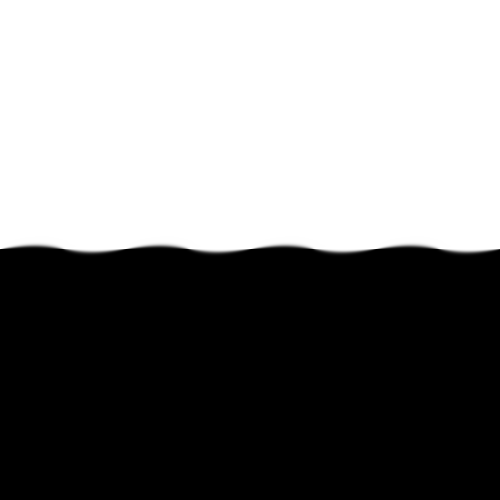
\includegraphics[width=9.2em]{run/images/20_steps.png}
  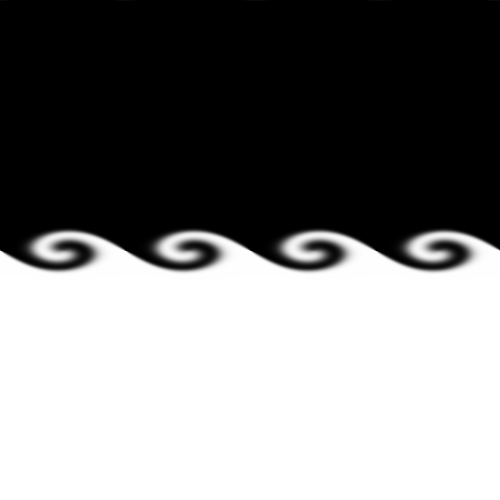
\includegraphics[width=9.2em]{run/images/100_steps.png}
  
\includegraphics[width=9.2em]{run/images/300_steps.png}
  
\includegraphics[width=9.2em]{run/images/500_steps.png}
  \caption{Evolution of the fluid flow after 20, 100, 300, and 500 simulation steps.
  Here white corresponds to the value where dye is at most intense whereas the black regions contain no dye at all.}
  \label{result}
\end{figure}
Figure \ref{result} shows the evolution of the fluid by applying the parameters given in the project instructions.
The initial forces are defined in such a way that \dots
As can be seen from the figure, in the beginning at 20 simulation steps the dye is almost unperturbed.
At 100 steps turbulent vortices are emerge.
At 300th step the initial vortices have almost dissipated with new vortices emerging at the edge where y-boundary is wrapped.
At 500th step new -- and larger -- vortices are emerging in the middle.

The nature of the flow can be changed significantly by adjusting the parameters
For instance, by increasing the viscosity, the fluid will instead stabilize after an initial perturbation.
Decreasing the viscosity on the other hand will tend to increase the instability as would be expected.
%Whether this is because of a bug in my code or just unstable behavior for small numerical values I am not sure.

\begin{figure}[h!]
  \center
  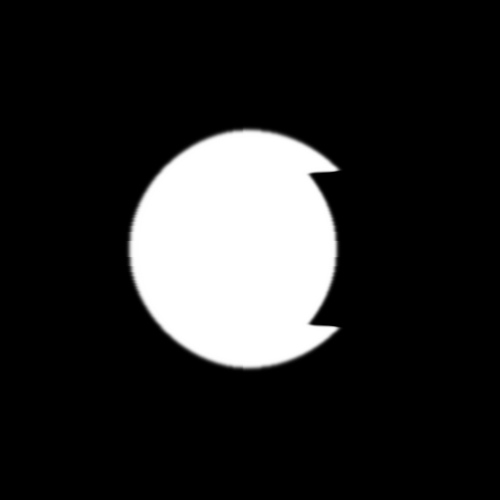
\includegraphics[width=9.2em]{run/images/20_Steps.png}
  
\includegraphics[width=9.2em]{run/images/100_Steps.png}
  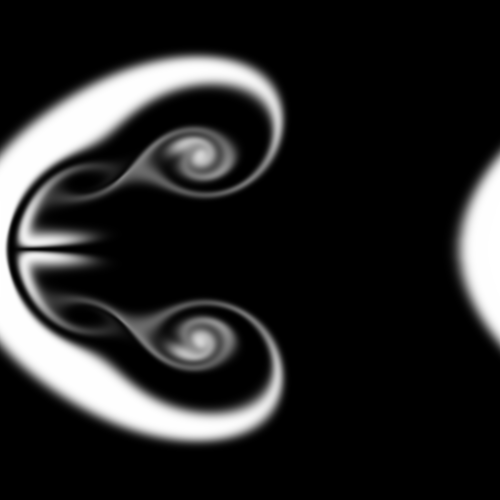
\includegraphics[width=9.2em]{run/images/300_Steps.png}
  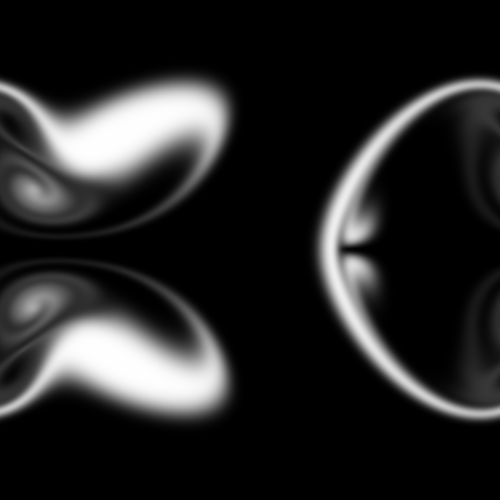
\includegraphics[width=9.2em]{run/images/500_Steps.png}
  \caption{Evolution of the fluid flow 20, 100, 300, and 500 simulation steps.
  A leftward force positioned at the central right of the blob is applied for 10 simulation steps}
  \label{result2}
\end{figure}
\pagebreak
I had also attempted to replicate the flowing blob of dye from the project instruction sheet.
This turned out to be a bit more difficult than I expected but I am quite happy with the result which is shown in the figure \ref{result2}.



For convenience, I implemented a function for applying a circular blob of dye by pressing the left mouse button.
This allows for a convenient way of stydying the behavior of the fluid.

\section{Conclusions}
The application of Stam's simulator seems to have been successful.
An initial force creates disturbances in the flow, resulting in occasional turbulent vortices and eventual mixing of the dye.
A demonstration of Kelvin-Helmholtz instability was successful and I learned a lot about fluid simulations through this project.
%An inclusion of scaling option for the rendered fluid could be helpful for screens with different resolution
%It could be interesting to try to implement an interaction of different fluids

The program could be extended to have a more streamlined method for interacting with the flow.
For instance, an external force could be then applied by right-clicking and dragging the cursor.
This would however be mostly a matter of convenience.
Possible extension for three-dimensional simulator should be fairly straight-forward.
Although an implementation of renderer for that three-dimensional fluid flow would probably be a nightmare.
%\printbibliography
\begin{thebibliography}{9}
  \bibitem{Stam1}
    Jos Stam. 2001. A Simple Fluid Solver Based on the FFT. Journal of Graphics Tools, 6(2), 43–52. https://doi.org/10.1080/10867651.2001.10487540
  \bibitem{Stam2}
    Jos Stam. 1999. Stable fluids. In Proceedings of the 26th annual conference on Computer graphics and interactive techniques (SIGGRAPH '99). ACM Press/Addison-Wesley Publishing Co., USA, 121–128. https://doi.org/10.1145/311535.311548
  \bibitem{SDL2}
    SDL, GitHub repository, https://github.com/libsdl-org/SDL
  \bibitem{Wiki}
    Kelvin–Helmholtz instability (2025, May 22). In Wikipedia. \\
    https://en.wikipedia.org/wiki/Kelvin\%E2\%80\%93Helmholtz\_instability
\end{thebibliography}

\end{document}

